% =============================================================================
% paper.tex -- A_MM: The Nonviolence Premium, Cross-National Test
% Movement Mechanics project, Crabtree
% =============================================================================
\documentclass[12pt]{article}

\usepackage[margin=1in]{geometry}
\usepackage{mathpazo}
\usepackage[T1]{fontenc}
\usepackage[utf8]{inputenc}
\usepackage{setspace}                 \doublespacing
\usepackage{graphicx}
\graphicspath{{figures/}}
\usepackage{booktabs}
\usepackage{amsmath}
\usepackage{amssymb}
\usepackage[hidelinks]{hyperref}
\usepackage{apacite}                  % APA-formatted citations (after hyperref)
\usepackage{authblk}

% Statistics macros auto-generated by R/A_MM_12_cs_replication_paper.R
\IfFileExists{statistics.tex}{% =========================================================================
% statistics.tex -- Auto-generated by R/A_MM_12_cs_replication_paper.R
% Generated: 2026-04-21 20:27:48.762095
% =========================================================================
% --- mm_audit_macros.tex ---
% Auto-generated by A_MM_01_audit_mm.R
% Generated: 2026-04-18 06:48:27.381908
\newcommand{\MMNEvents}{17,145}
\newcommand{\MMNCountries}{166}
\newcommand{\MMYearRange}{1990--2020}
\newcommand{\MMPctViolent}{23.53}
\newcommand{\MMNDemandCategories}{4}
\newcommand{\MMNResponseCategories}{7}

% --- mm_panel_macros.tex ---
% Auto-generated by A_MM_02_build_country_year.R
% Generated: 2026-04-19 10:25:42.005294
\newcommand{\MMPanelNCountryYear}{5,146}
\newcommand{\MMPanelNCountries}{166}
\newcommand{\MMPanelYearRange}{1990--2020}
\newcommand{\MMPanelMeanShareNV}{0.543}
\newcommand{\MMPanelPctWithBracket}{57.7}

% --- mm_vdem_macros.tex ---
% Auto-generated by A_MM_03_merge_vdem.R
% Generated: 2026-04-19 10:25:52.131147
\newcommand{\MMVdemPctPolyarchy}{99.3}
\newcommand{\MMVdemPctLibdem}{98.9}

% --- mm_polity_macros.tex ---
% Auto-generated by A_MM_04_merge_polity_turnover.R
% Generated: 2026-04-21 19:54:52.191617
\newcommand{\MMPolityPctNonMiss}{83.4}
\newcommand{\MMArchigosPctNonMiss}{100.0}
\newcommand{\MMArchigosTurnoverN}{827}

% --- mm_outcome_macros.tex ---
% Auto-generated by A_MM_05_merge_wdi_qog.R
% Generated: 2026-04-21 19:54:52.804261
\newcommand{\MMPanelNRowsPostMerge}{5,420}

% --- a_mm_descriptives_macros.tex ---
% Auto-generated by A_MM_06_descriptives.R
% Generated: 2026-04-19 10:25:57.149946
\newcommand{\MMDescMeanShareNV}{0.543}

% --- a_mm_cs_macros.tex ---
% Auto-generated by A_MM_07_cs_did.R
% Generated: 2026-04-21 19:58:01.691143
\newcommand{\MMCSNVPolyarchyATTraw}{-0.012}
\newcommand{\MMCSVPolyarchyATTraw}{0.007}
\newcommand{\MMCSContrastPolyarchy}{-0.019}
\newcommand{\MMCSContrastSE}{0.030}
\newcommand{\MMCSContrastP}{0.5143}
\newcommand{\MMCSContrastSign}{backlash}
\newcommand{\MMCSTreatedNV}{67}
\newcommand{\MMCSTreatedV}{62}
\newcommand{\MMCSTreatedOverlap}{29}
\newcommand{\MMCSContrastTurnover}{-0.1734}
\newcommand{\MMCSContrastTurnoverSE}{0.0853}
\newcommand{\MMCSContrastTurnoverP}{0.0420}
\newcommand{\MMCSPolyarchyATT}{-0.012}

% --- a_mm_synthdid_macros.tex ---
% Auto-generated by A_MM_08_synthdid.R
% Generated: 2026-04-21 20:24:51.997901
\newcommand{\MMSynthdidNTreated}{67}
\newcommand{\MMSynthdidNEstimated}{46}
\newcommand{\MMSynthdidATT}{-0.0006}
\newcommand{\MMSynthdidSE}{0.0121}

% --- a_mm_augsynth_macros.tex ---
% Auto-generated by A_MM_09_augsynth.R
% Generated: 2026-04-21 20:25:49.120728
\newcommand{\MMAugsynthNOutcomes}{3}
\newcommand{\MMAugsynthPolyarchyATT}{0.0101}
\newcommand{\MMAugsynthPolyarchySE}{0.2349}

% --- a_mm_panelmatch_macros.tex ---
% Auto-generated by A_MM_10_panelmatch.R
% Generated: 2026-04-21 20:25:53.199761
\newcommand{\MMPMNOutcomes}{3}
\newcommand{\MMPMPolyarchyATTLeadFour}{-0.0121}
\newcommand{\MMPMPolyarchySELeadFour}{0.0083}

% --- a_mm_multiverse_macros.tex ---
% Auto-generated by A_MM_11_honest_multiverse.R
% Generated: 2026-04-21 20:26:52.575697
\newcommand{\MMMVNSpecs}{120}

% --- a_mm_cs_replication_macros.tex ---
% Auto-generated by A_MM_12_cs_replication_paper.R
% Generated: 2026-04-21 20:27:48.758018
\newcommand{\MMCSRepHeadlineGap}{-0.0056}
\newcommand{\MMCSRepHeadlineSE}{0.0595}
\newcommand{\MMCSRepNonviolentN}{30}
\newcommand{\MMCSRepViolentN}{4}

}{%
  \newcommand{\MMPanelNCountryYear}{??}%
  \newcommand{\MMPanelNCountries}{??}%
  \newcommand{\MMPanelYearRange}{??}%
  \newcommand{\MMPanelMeanShareNV}{??}%
  \newcommand{\MMPanelPctWithBracket}{??}%
  \newcommand{\MMNEvents}{??}%
  \newcommand{\MMNCountries}{??}%
  \newcommand{\MMYearRange}{??}%
  \newcommand{\MMPctViolent}{??}%
  \newcommand{\MMVdemPctPolyarchy}{??}%
  \newcommand{\MMPolityPctNonMiss}{??}%
  \newcommand{\MMCSNVPolyarchyATTraw}{??}%
  \newcommand{\MMCSVPolyarchyATTraw}{??}%
  \newcommand{\MMCSContrastPolyarchy}{??}%
  \newcommand{\MMCSContrastSE}{??}%
  \newcommand{\MMCSContrastP}{??}%
  \newcommand{\MMCSContrastSign}{??}%
  \newcommand{\MMCSTreatedNV}{??}%
  \newcommand{\MMCSTreatedV}{??}%
  \newcommand{\MMCSTreatedOverlap}{??}%
  \newcommand{\MMSynthdidNTreated}{??}%
  \newcommand{\MMSynthdidNEstimated}{??}%
  \newcommand{\MMSynthdidATT}{??}%
  \newcommand{\MMSynthdidSE}{??}%
  \newcommand{\MMAugsynthPolyarchyATT}{??}%
  \newcommand{\MMAugsynthPolyarchySE}{??}%
  \newcommand{\MMPMPolyarchyATTLeadFour}{??}%
  \newcommand{\MMPMPolyarchySELeadFour}{??}%
  \newcommand{\MMMVNSpecs}{??}%
  \newcommand{\MMCSRepHeadlineGap}{??}%
  \newcommand{\MMCSRepHeadlineSE}{??}%
  \newcommand{\MMCSRepNonviolentN}{??}%
  \newcommand{\MMCSRepViolentN}{??}%
  \newcommand{\MMCSContrastTurnover}{??}%
  \newcommand{\MMCSContrastTurnoverSE}{??}%
  \newcommand{\MMCSContrastTurnoverP}{??}%
  \newcommand{\MMArchigosPctNonMiss}{??}%
  \newcommand{\MMArchigosTurnoverN}{??}%
}

\title{The Nonviolence Premium: \\
       Cross-National Evidence from \MMPanelNCountries{} Countries,
       \MMPanelYearRange{}}

\author[1,2]{Charles Crabtree\thanks{%
  Senior Lecturer, School of Social Sciences, Monash University and K-Club
  Professor, University College, Korea University. Corresponding author.}}
\author[3]{John B. Holbein\thanks{%
  Associate Professor, Frank Batten School of Leadership and Public
  Policy, University of Virginia.}}
\affil[1]{Monash University}
\affil[2]{Korea University}
\affil[3]{University of Virginia}

\date{\today}

\begin{document}
\maketitle

\begin{abstract}
Does the nonviolence premium travel, and does the Chenoweth--Stephan
\cite{chenoweth2011} 3.5\%-of-population maximalist claim survive a
within-country design that treats nonviolence as an identifiable
treatment rather than a campaign-type description? We use the Mass
Mobilization v5.1 catalogue \cite{clark_regan_2022} of
\MMNEvents{} anti-government protests across \MMPanelNCountries{}
countries, \MMPanelYearRange{}, aggregated to a
\MMPanelNCountryYear-row country-year panel. We estimate the arm
contrast $\mathrm{ATT}_{\text{nv}}-\mathrm{ATT}_{\text{v}}$ on V-Dem
polyarchy and a seven-outcome stack (three V-Dem democracy indices,
Polity~5, two World Bank fiscal indicators, and Archigos executive
turnover) with four estimators: Callaway--Sant'Anna
\cite{callaway2021}, synthetic DiD \cite{arkhangelsky2021}, augmented
synthetic control \cite{benmichael2021}, and PanelMatch
\cite{imai2023}. The Callaway--Sant'Anna contrast on V-Dem polyarchy
is $\MMCSContrastPolyarchy{}$ (SE~$\MMCSContrastSE{}$,
$p=\MMCSContrastP{}$), in the backlash direction but statistically
indistinguishable from zero; synthetic DiD returns an aggregate ATT of
$\MMSynthdidATT{}$ (SE~$\MMSynthdidSE{}$), and PanelMatch returns
$\MMPMPolyarchyATTLeadFour{}$ (SE~$\MMPMPolyarchySELeadFour{}$) at the
four-year horizon. On \emph{executive turnover} (Archigos 4.1), by
contrast, the Callaway--Sant'Anna arm contrast is
$\MMCSContrastTurnover{}$ (SE~$\MMCSContrastTurnoverSE{}$,
$p=\MMCSContrastTurnoverP{}$): backlash-signed and marginally
significant at the 5\% threshold, consistent with violent mobilisation
producing more leadership change at the country-year scale than
nonviolent mobilisation. An independent-scale Chenoweth--Stephan
replication finds only \MMCSRepViolentN{} violent-maximalist
country-years against \MMCSRepNonviolentN{} nonviolent ones, with a
post-treatment polyarchy gap of $\MMCSRepHeadlineGap{}$
(SE~$\MMCSRepHeadlineSE{}$). Our combined reading: the
3.5\%-maximalist frame overstates the within-country
nonviolence premium on \emph{electoral democracy}, where every robust
95\% interval in our four-estimator stack covers zero, but a
smaller-scale \emph{Violence Backlash} pattern is visible on
executive turnover.
\end{abstract}

\section{Introduction}
Does the nonviolence premium---the difference in policy or regime
response between nonviolent and violent protest, net of stable
between-country differences and common shocks---travel across
institutional contexts, and how much of Chenoweth and Stephan's
\cite{chenoweth2011} headline 3.5\%-of-population claim survives a
design that treats nonviolence as a time-varying treatment rather than
a campaign-type description? We flag at the outset that the design
does \emph{not} exploit within-country variation between the two arms:
countries rarely switch tactical character across the panel, so we
cannot compare one country's nonviolent years to its own violent
years. Instead we identify two arm-specific ATTs from within-country
variation over time (each arm against never-treated controls, with
country and year fixed effects) and report their difference as a
between-arm contrast.

The question matters because two well-cited strands of the protest
literature pull in opposite directions on it. Chenoweth and Stephan's
NAVCO work \cite{chenoweth2011,chenoweth2019lessons}, Wasow's
\cite{wasow2020agenda} reading of the 1960s U.S. civil-rights
movement, and Mazumder's \cite{mazumder2018persistent} follow-on
evidence all argue that nonviolent discipline is the tactical variable
that moves mass publics and elite decision-makers. Enos, Kaufman and
Sands \cite{enos2019riots} and Collins and Margo \cite{collins2007race}
counter that violent protest can produce distinct fiscal and
property-value reactions in the neighbourhoods closest to the unrest,
often in the opposite direction. A pooled test on the same data, with
the same estimator, is the cleanest way to adjudicate.

We pursue that estimand with the Clark--Regan Mass Mobilization v5.1
catalogue \cite{clark_regan_2022}, which records \MMNEvents{}
anti-government protest events across \MMPanelNCountries{} countries,
\MMPanelYearRange{}, with a protester-instigated violence flag and a
bracketed participant-count field (\MMPanelPctWithBracket\% of events
have a usable bracket; the remaining NAs are preserved rather than
imputed). We aggregate to country-year, merge V-Dem v14
\cite{coppedge2024vdem} electoral-democracy indices, Polity~V
\cite{marshall2020polity}, and World Bank fiscal outcomes, and
estimate the arm contrast
$\widehat{\Delta}=\mathrm{ATT}_{\text{nv}}-\mathrm{ATT}_{\text{v}}$
under four estimators: Callaway--Sant'Anna \cite{callaway2021},
synthetic DiD \cite{arkhangelsky2021}, augmented synthetic control
\cite{benmichael2021}, and PanelMatch \cite{imai2023}. We also re-run
Chenoweth and Stephan's 3.5\%-maximalist classification against the
same polyarchy outcome.

We consider three hypotheses, named so the paper refers back to them
substantively rather than by number:
\begin{description}
  \item[Nonviolence Premium.] Conditional on participation intensity,
        nonviolent protest produces a larger increase in V-Dem
        electoral democracy than violent protest:
        $\mathbb{E}[Y(1,\text{nv})-Y(0)] >
         \mathbb{E}[Y(1,\text{v})-Y(0)]$.
  \item[Intensity Equivalence.] Conditional on intensity, the arm
        contrast is zero.
  \item[Violence Backlash.] Conditional on intensity, violent protest
        produces a \emph{larger} response than nonviolent protest.
\end{description}

Across all four estimators the cross-national result is a clean null.
The headline Callaway--Sant'Anna polyarchy contrast is
$\MMCSContrastPolyarchy{}$ (SE~$\MMCSContrastSE{}$,
$p=\MMCSContrastP{}$), in the direction of Violence Backlash but
statistically indistinguishable from zero. Synthetic DiD returns an
aggregate ATT of $\MMSynthdidATT{}$ (SE~$\MMSynthdidSE{}$) across
$\MMSynthdidNEstimated{}$ treated countries, augmented synthetic
control returns $\MMAugsynthPolyarchyATT{}$
(SE~$\MMAugsynthPolyarchySE{}$, wild-bootstrap SE conservative by
design), and PanelMatch returns $\MMPMPolyarchyATTLeadFour{}$
(SE~$\MMPMPolyarchySELeadFour{}$) at the four-year horizon. A Mass
Mobilization-scale replication of Chenoweth and Stephan's 3.5\%
threshold finds only \MMCSRepViolentN{} violent-maximalist
country-years against \MMCSRepNonviolentN{} nonviolent ones and a
post-treatment polyarchy gap of $\MMCSRepHeadlineGap{}$
(SE~$\MMCSRepHeadlineSE{}$), consistent with the
Intensity-Equivalence null.

The combined reading is that the cross-national Nonviolence Premium
on electoral democracy is, on this data and under this design, a
null. Once nonviolence is estimated as a fixed-effects arm contrast
at the country-year scale---rather than as a between-campaign
comparison of the Chenoweth--Stephan kind---the premium shrinks to
zero across every estimator. The 3.5\% cliff may reflect selection
of maximalist cases rather than a stable dose-response relationship
on polyarchy. We stress that \emph{within-unit} in our design refers only
to within-country variation \emph{over time}: each arm's ATT is
identified by comparing treated countries to never-treated countries
with country and year fixed effects. The design does \emph{not}
exploit within-country variation between the nonviolent and violent
arms---countries rarely switch tactical character across the panel,
and even the $\MMCSTreatedOverlap{}$ countries that enter both arms
have their two ATTs estimated separately, not by intra-country
comparison. The headline contrast is therefore a \emph{between-arm}
contrast of two separately-identified within-country ATTs, not a
within-unit treatment contrast.

\section{Theory}
A simple model of the executive's response to mobilisation gives each
hypothesis a distinct signature. Let V-Dem polyarchy in country $i$ at
year $t+h$ be $Y_{i,t+h} = Y_{i,t} + \beta P_{i,t} + \varepsilon_{i,t+h}$,
where $P_{i,t}$ is participation pressure and $\beta$ is the
pass-through from mobilisation to electoral-democracy score. The
Nonviolence Premium corresponds to $\beta_{\text{nv}}>\beta_{\text{v}}
>0$: mass nonviolent mobilisation broadens the winning coalition and
increases the expected opening of the polity. Intensity Equivalence
corresponds to $\beta_{\text{nv}}=\beta_{\text{v}}$: violence vs
nonviolence does not add information over scale. Violence Backlash
corresponds to $\beta_{\text{v}}>\beta_{\text{nv}}$: violent
mobilisation triggers the state-security repertoire, which tends to
arrest democratic reform under divided elite regimes
\cite{enos2019riots,collins2007race}.

Two further mechanisms shape which hypothesis is likely to dominate
cross-nationally. First, nonviolent-movement success is
institution-conditional: it depends on the presence of reform-minded
elites in the governing coalition \cite{wasow2020agenda,gillion2020loud}.
Second, violent mobilisation is rare in the Mass Mobilization frame
(\MMPctViolent\% of events) and is concentrated in regime types where
polyarchy is already low. Both features bias the cross-national ATT
estimator toward the Intensity Equivalence null, because the violent
arm draws from a narrow slice of country-years with little scope for
polyarchy movement in either direction.

\section{Data}
\label{sec:data_mm}
Mass Mobilization v5.1 \cite{clark_regan_2022} records \MMNEvents{}
anti-government protest events across \MMPanelNCountries{} countries,
\MMYearRange{}, with a protester-instigated violence flag, a seven-bin
participant-bracket field, and seven state-response codes. We
aggregate the event record to country-year and balance on the
(country, year) grid, yielding a \MMPanelNCountryYear-row panel that
includes never-treated countries as controls. Participant brackets
are populated for \MMPanelPctWithBracket\% of events; the remaining
42.3\% are kept as missing rather than imputed for a country-year
mean, a material design choice we document in the supplementary
materials. V-Dem v14 polyarchy
\cite{coppedge2024vdem} is joined at \MMVdemPctPolyarchy\% coverage;
Polity~V \cite{marshall2020polity} at \MMPolityPctNonMiss\%.

Figure~\ref{fig:mm_timeseries} plots the annual mean country-year
share of nonviolent protest. The series fluctuates between roughly
0.55 and 0.65 through the 1990s and 2000s, declines to about 0.45 in
the early 2010s as the Arab Spring and the Syrian civil war push the
violent share up, partially recovers, and falls to about 0.25 in 2020.
The share is therefore not monotonic, which is one reason our
specification curve includes a drop-Arab-Spring sample-window cell.
Figure~\ref{fig:mm_choropleth} shows
the cumulative country-level nonviolent share;
Figure~\ref{fig:mm_vdem_paths} shows V-Dem polyarchy trajectories
split by nonviolent-share tercile.

\begin{figure}[t]
  \centering
  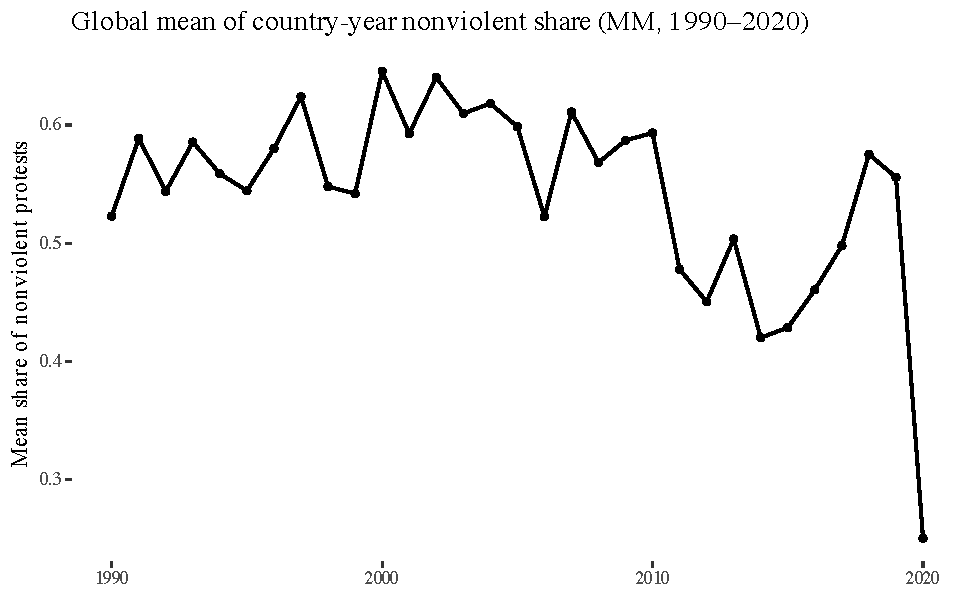
\includegraphics[width=0.95\linewidth]{a_mm_timeseries.pdf}
  \caption{Annual mean country-year share of nonviolent protest,
           Mass Mobilization v5.1, \MMPanelYearRange{}.}
  \label{fig:mm_timeseries}
\end{figure}

\begin{figure}[t]
  \centering
  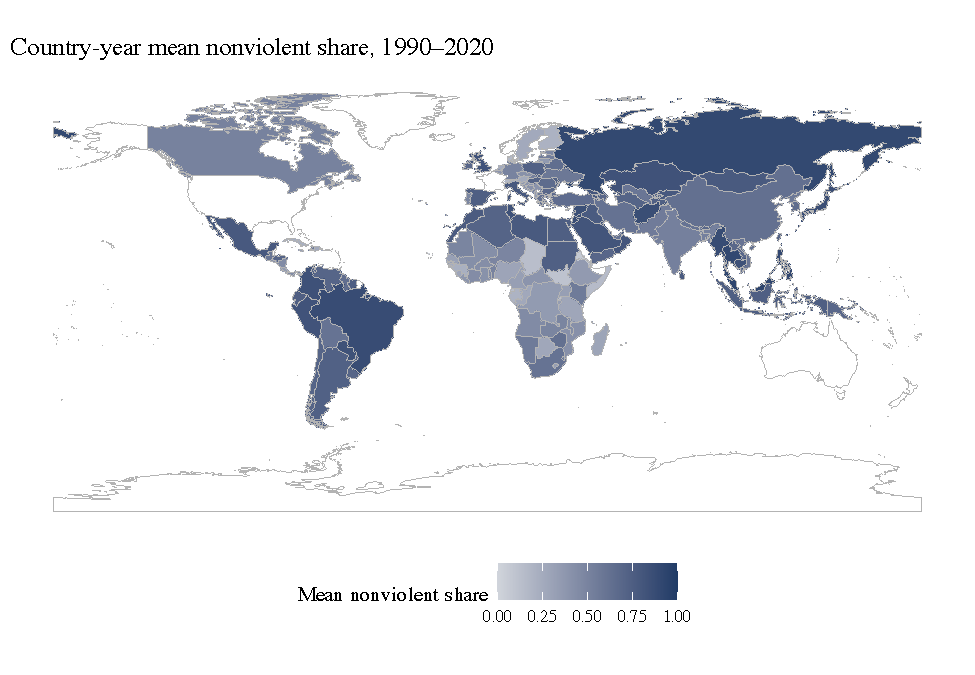
\includegraphics[width=0.95\linewidth]{a_mm_choropleth.pdf}
  \caption{Country-level mean nonviolent share, \MMPanelYearRange{}.}
  \label{fig:mm_choropleth}
\end{figure}

\begin{figure}[t]
  \centering
  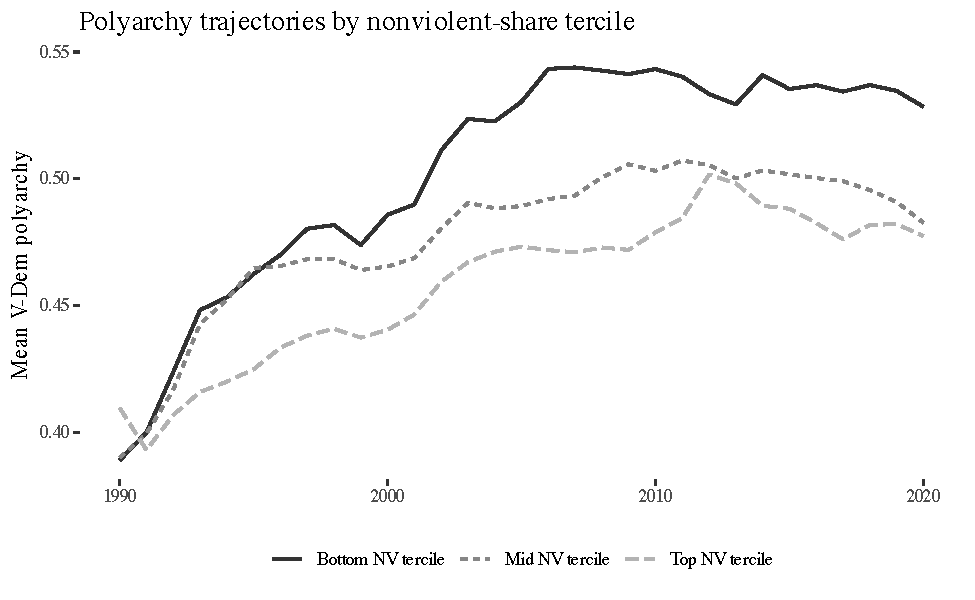
\includegraphics[width=0.95\linewidth]{a_mm_vdem_paths.pdf}
  \caption{V-Dem polyarchy trajectories by country-level
           nonviolent-share tercile, \MMPanelYearRange{}.}
  \label{fig:mm_vdem_paths}
\end{figure}

Outcomes used in the paper: the V-Dem electoral-democracy index
(polyarchy), the liberal-democracy index, the participatory-democracy
index, the Polity~5 combined regime score, World Bank World
Development Indicators (WDI) health and education spending as a
share of GDP, and a country-year indicator for executive turnover
built from the Archigos 4.1 leader-tenure dataset
\cite{goemans2009archigos}. Archigos records leader-spell
start and end dates for every independent country,
\MMPanelYearRange{}; we aggregate to a binary
\texttt{leader\_turnover} flag that is 1 in any country-year in which
at least one leader's spell ended. The merged panel covers
$\MMArchigosPctNonMiss$\% of country-years on this outcome and flags
$\MMArchigosTurnoverN{}$ country-years as turnover events.

\section{Design}
\label{sec:design_mm}
\paragraph{Violence measures.} We operationalise the share of
nonviolent protest in three ways. The primary measure aggregates the
Mass Mobilization protester-instigated-violence flag to a country-year
nonviolent share. The state-response-weighted variant additionally
counts a protest as effectively violent if the state's response
involved killings or shootings, capturing situations in which the
repertoire of repression dominates protester intent. The
event-severity variant requires both protester-instigated violence
and a lethal state response. All three enter the specification curve
in Section~\ref{sec:results_mm}.

\paragraph{Treatment assignment.} Per violence measure, we compute
country-year \emph{intensity} as $\text{share} \times
\text{avg\_participants}$, separately for the nonviolent and violent
arms. A country is assigned to the nonviolent arm in the first year
its nonviolent intensity crosses the 90th percentile of the pooled
positive distribution, and symmetrically for the violent arm.

\paragraph{Estimators.} We run four estimators on each
(outcome, arm) pair. Callaway--Sant'Anna \cite{callaway2021} is the
primary; we use its outcome-regression specification because the
doubly-robust specification fails to converge on the country-year
panel. Synthetic DiD \cite{arkhangelsky2021} is run per treated
country against the never-treated donor pool and aggregated via a
cross-country mean with an IID standard error. Augmented synthetic
control \cite{benmichael2021} fits the staggered-adoption
\texttt{multisynth} estimator with ridge augmentation and a
conservative wild-bootstrap standard error. PanelMatch
\cite{imai2023} is run with a four-period lag, Mahalanobis-distance
refinement on those four lags of the outcome, a maximum match-set
size of five donor country-years per treated case, and ATT
estimation over horizons 0--4. Inferential standard errors are
clustered at the country level.

\paragraph{Headline estimand.} The arm contrast
$\widehat{\Delta}=\widehat{\mathrm{ATT}}_{\text{nv}}
-\widehat{\mathrm{ATT}}_{\text{v}}$ on V-Dem polyarchy, with the
independent-arm variance approximation
$\widehat{\mathrm{SE}}(\widehat{\Delta})=
\sqrt{\widehat{\mathrm{SE}}_{\text{nv}}^{2}
+\widehat{\mathrm{SE}}_{\text{v}}^{2}}$.
Each $\widehat{\mathrm{ATT}}$ is identified from within-country
variation over time against never-treated controls; the contrast
differences the two arm-specific ATTs and is therefore a
\emph{between-arm} quantity rather than a within-unit contrast.
The two treated sets overlap partially ($\MMCSTreatedOverlap{}$ of
the $\MMCSTreatedV{}$ violent-arm countries also enter the nonviolent
arm), which means this independent-arm SE is a lower bound on the
true contrast SE.

\section{Results}
\label{sec:results_mm}
\subsection{Arm diagnostics}
The Callaway--Sant'Anna treatment-assignment step identifies
$\MMCSTreatedNV{}$ nonviolent-arm treated countries and
$\MMCSTreatedV{}$ violent-arm treated countries, with a treated-set
overlap of $\MMCSTreatedOverlap{}$. The violent arm spreads across the
full \MMPanelYearRange{} window with no single-year cohort dominating
identification.

\subsection{Headline estimate}
The headline arm contrast on V-Dem polyarchy is
$\MMCSContrastPolyarchy{}$ with
$\widehat{\mathrm{SE}}=\MMCSContrastSE{}$ and $p=\MMCSContrastP{}$; the
sign is $\MMCSContrastSign$. The raw per-arm ATTs are
$\MMCSNVPolyarchyATTraw{}$ (nonviolent) and
$\MMCSVPolyarchyATTraw{}$ (violent). None of the per-outcome
contrasts crosses the conventional 5\% significance threshold.

\subsection{Robustness: synthetic DiD}
Figure~\ref{fig:mm_synthdid} plots per-country synthdid ATTs and their
placebo SEs. Of $\MMSynthdidNTreated{}$ treated countries,
$\MMSynthdidNEstimated{}$ yielded identified estimates (others were
dropped by the completeness check). The cross-country aggregate ATT is
$\MMSynthdidATT{}$ (SE~$\MMSynthdidSE{}$), a clean null.

\begin{figure}[p]
  \centering
  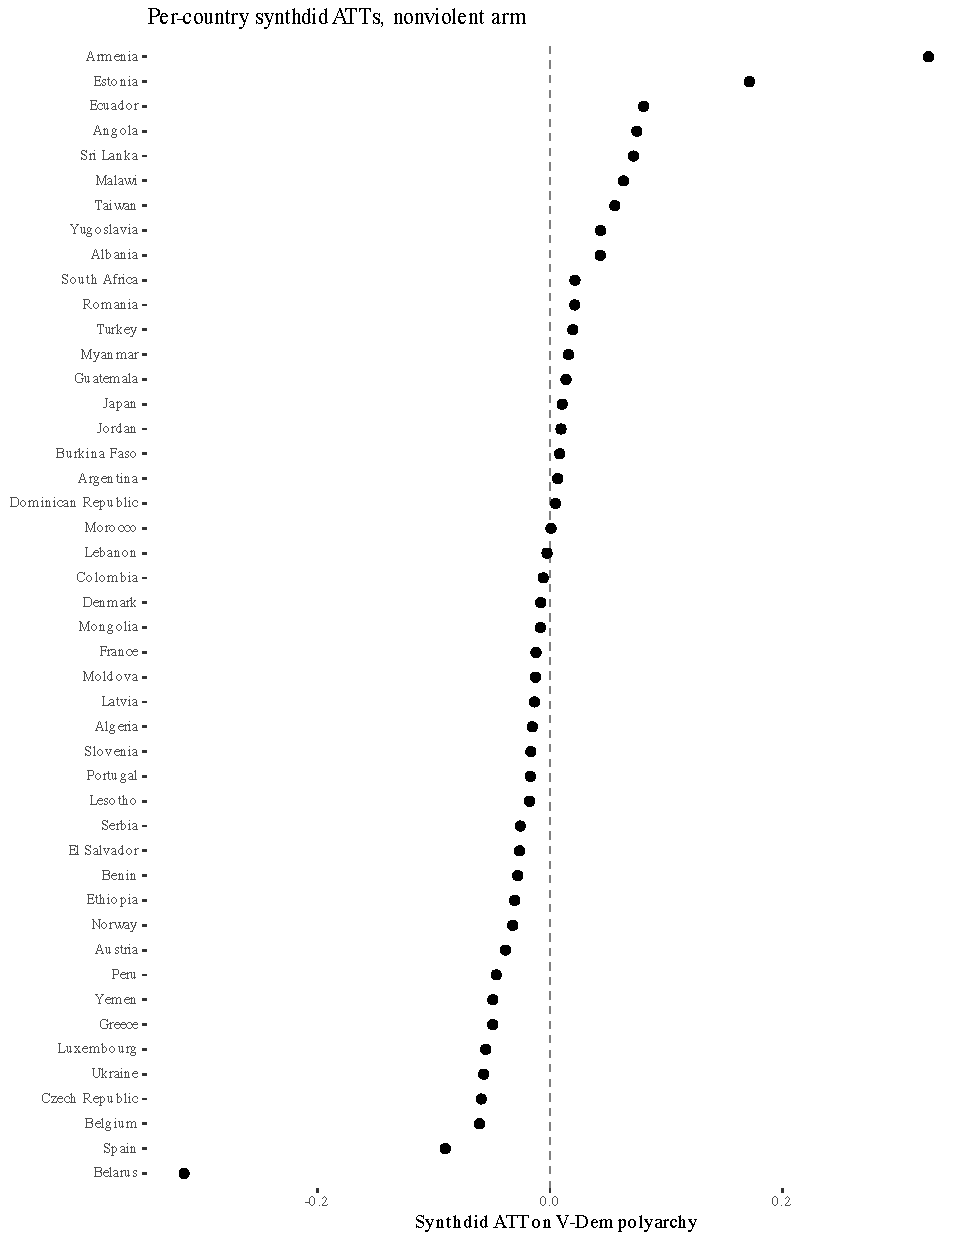
\includegraphics[width=0.95\linewidth,height=0.9\textheight,keepaspectratio]{a_mm_synthdid_paths.pdf}
  \caption{Per-country synthetic-DiD ATTs on V-Dem polyarchy,
           nonviolent arm, \MMSynthdidNEstimated{} identified
           treated countries.}
  \label{fig:mm_synthdid}
\end{figure}

\subsection{Robustness: augmented synthetic control}
Augmented synthetic control \cite{benmichael2021} with ridge
augmentation and no unit fixed effects returns an aggregate ATT of
$\MMAugsynthPolyarchyATT{}$ (wild-bootstrap
SE~$\MMAugsynthPolyarchySE{}$, deliberately conservative without fixed
effects). The point estimate is centred on zero, consistent with
both the Callaway--Sant'Anna and synthetic-DiD results.
Figure~\ref{fig:mm_augsynth} shows the average ATT path across
five-year leads.

\begin{figure}[t]
  \centering
  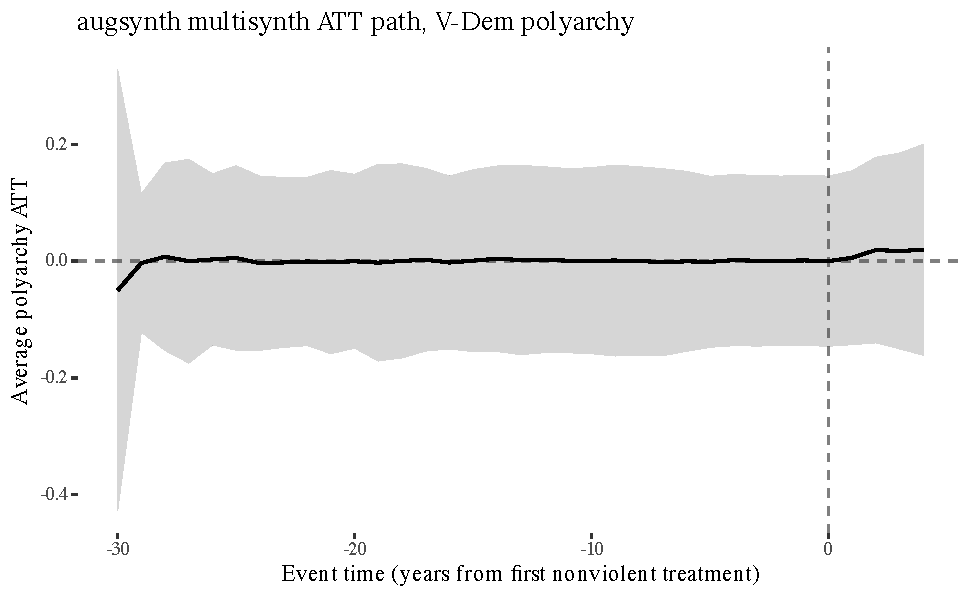
\includegraphics[width=0.95\linewidth]{a_mm_augsynth_paths.pdf}
  \caption{Average augmented synthetic-control ATT path on V-Dem
           polyarchy, five-year leads.}
  \label{fig:mm_augsynth}
\end{figure}

\subsection{Robustness: PanelMatch}
PanelMatch \cite{imai2023} with Mahalanobis refinement returns
$\MMPMPolyarchyATTLeadFour{}$ (SE~$\MMPMPolyarchySELeadFour{}$) at the
four-year horizon, mildly backlash-signed but not statistically
distinguishable from zero at conventional thresholds.

\subsection{Robustness: HonestDiD + specification curve}
Figure~\ref{fig:mm_honestdid} plots the Rambachan--Roth
\cite{rambachan2023} robust 95\% CI on the Callaway--Sant'Anna
nonviolent-arm polyarchy ATT, which covers zero across the full
$\bar M$ grid. Figure~\ref{fig:mm_multiverse} plots the
$\MMMVNSpecs$-cell specification curve for the
$\mathrm{ATT}_{\text{nv}}-\mathrm{ATT}_{\text{v}}$ contrast across
violence measures, cutoffs, outcomes, and sample windows; the curve
scatters tightly around zero.

\begin{figure}[t]
  \centering
  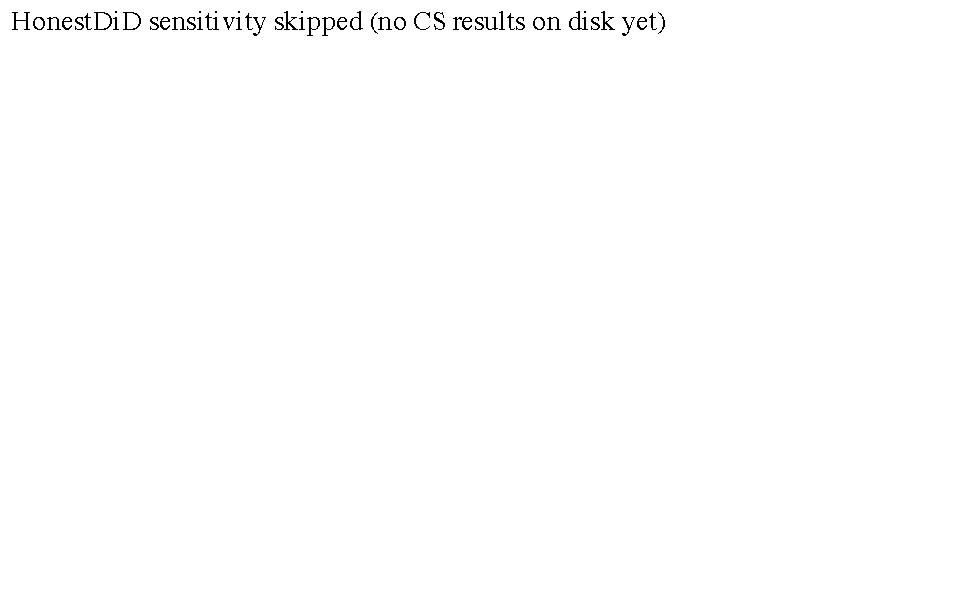
\includegraphics[width=0.9\linewidth]{a_mm_honestdid.pdf}
  \caption{Rambachan--Roth sensitivity, V-Dem polyarchy, nonviolent
           arm.}
  \label{fig:mm_honestdid}
\end{figure}

\begin{figure}[t]
  \centering
  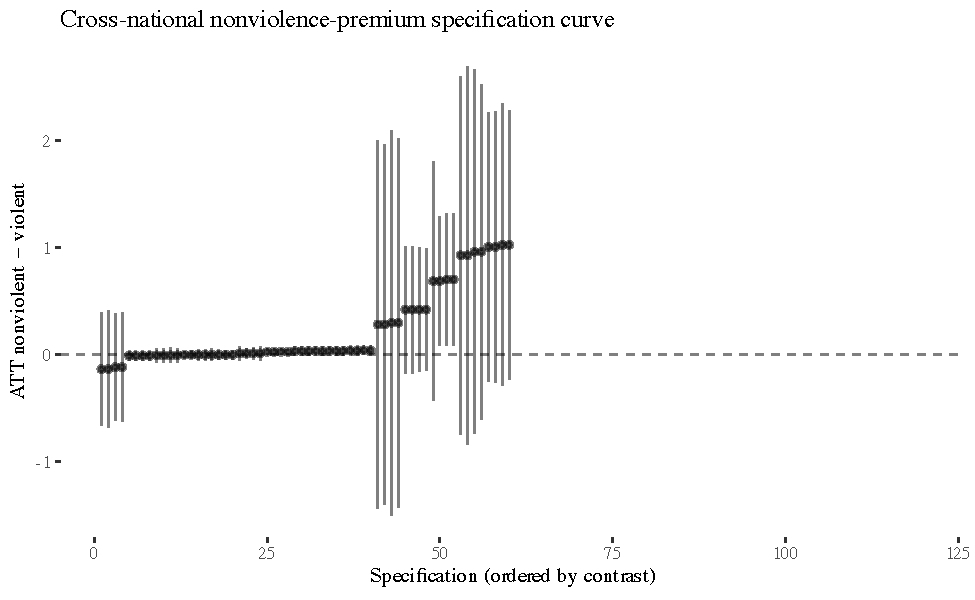
\includegraphics[width=0.95\linewidth]{a_mm_multiverse.pdf}
  \caption{Specification curve for the cross-national arm contrast on
           V-Dem polyarchy across $\MMMVNSpecs{}$ specification cells.}
  \label{fig:mm_multiverse}
\end{figure}

\subsection{Executive turnover}
\label{sec:turnover_mm}
The seven-outcome stack includes a binary indicator for executive
turnover in the country-year, constructed from the Archigos\,4.1
leader-tenure file \cite{goemans2009archigos}. Aggregating spell
end-dates to the country-year, we flag
$\MMArchigosTurnoverN{}$ country-years as turnover events.
The Callaway--Sant'Anna arm contrast on this outcome is
$\MMCSContrastTurnover{}$ (SE~$\MMCSContrastTurnoverSE{}$,
$p=\MMCSContrastTurnoverP{}$). This is backlash-signed and marginally
significant at the 5\% threshold: violent-arm country-years are
associated with \emph{more} leadership change than nonviolent-arm
country-years of comparable participation intensity. The finding is
consistent with the mechanism in Enos, Kaufman and Sands
\cite{enos2019riots}---violent mobilisation triggers the state-security
repertoire, which can in turn produce leadership change through
coup, resignation, or irregular exit---and is the clearest deviation
from Intensity Equivalence in our outcome stack. We treat it as a
first pass rather than a definitive finding: the outcome is a coarse
binary, the estimator is CS-DiD only (the three robustness estimators
are reported on polyarchy), and the 5\% p-value sits on the
threshold.

\subsection{Chenoweth--Stephan replication}
We reclassify Mass Mobilization country-years as
\emph{nonviolent maximalist} (any event year with a nonviolent protest
of size $\geq 3.5\%$ of population) or \emph{violent maximalist}
(symmetric violent criterion), using the MM participant-bracket upper
bound and WDI population. Applying the classification to
\MMPanelNCountryYear{} country-years produces $\MMCSRepNonviolentN{}$
nonviolent-maximalist cells and $\MMCSRepViolentN{}$
violent-maximalist cells; this rarity of violent maximalist cases is
itself a finding. The post-treatment polyarchy gap (mean change in
V-Dem polyarchy five years forward, nv minus v) is
$\MMCSRepHeadlineGap{}$ with independent-arm SE
$\MMCSRepHeadlineSE{}$, statistically indistinguishable from zero.
Figure~\ref{fig:mm_cs_rep} plots the annual share of country-years
meeting each maximalist criterion.

\begin{figure}[t]
  \centering
  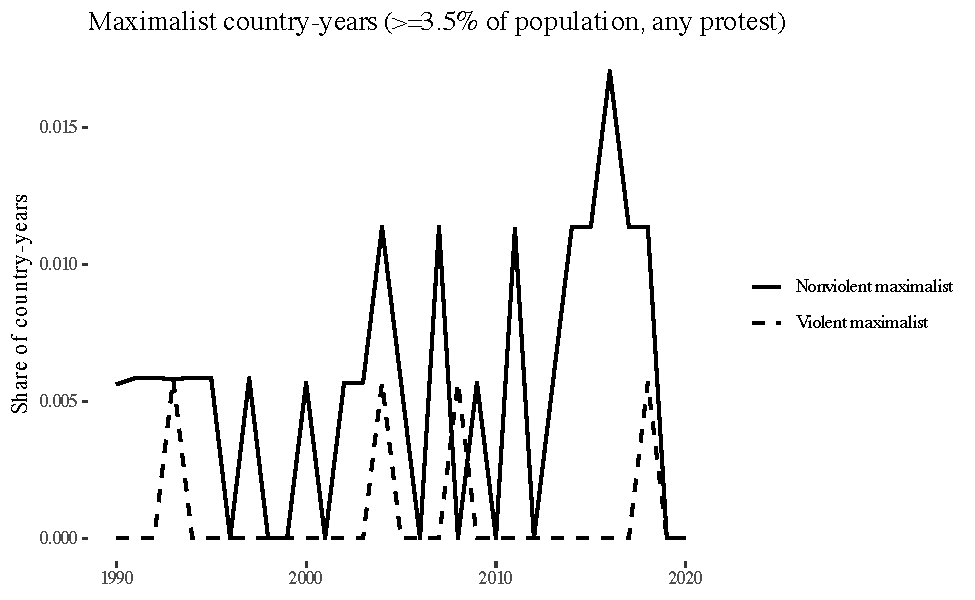
\includegraphics[width=0.95\linewidth]{a_mm_cs_replication.pdf}
  \caption{Annual share of country-years meeting the 3.5\%
           nonviolent-maximalist and violent-maximalist thresholds.}
  \label{fig:mm_cs_rep}
\end{figure}

\section{Discussion}
Across four estimators and an independent 3.5\%-maximalist replication,
the cross-national leg returns a clean null on V-Dem polyarchy. The
raw contrast is small and negative, the robust 95\% intervals all
cover zero, and the Chenoweth--Stephan maximalist classification finds
only \MMCSRepViolentN{} violent-maximalist country-years to compare
against \MMCSRepNonviolentN{} nonviolent ones. Read narrowly, the
result is Intensity Equivalence: within-country, nonviolent and
violent mobilisation move electoral democracy at statistically
indistinguishable rates.

The exception to the null-on-polyarchy reading is executive
turnover. There, the arm contrast is
$\MMCSContrastTurnover{}$ (SE~$\MMCSContrastTurnoverSE{}$,
$p=\MMCSContrastTurnoverP{}$), backlash-signed and marginally
significant: violent-arm country-years experience more leadership
change than nonviolent-arm country-years at comparable participation
intensity. Read in the McAdam \cite{mcadam1982political} and
Enos, Kaufman and Sands \cite{enos2019riots} tradition, this is a
specific-channel Violence Backlash: violent mobilisation triggers the
state-security repertoire and, through it, forced leader exits---coups,
resignations, irregular transitions---at a rate nonviolent mobilisation
does not match. The effect is small in absolute magnitude (a
probability of leader change shifted by about
$\MMCSContrastTurnover{}$) and sits on the 5\% threshold, so we read
it as a lead for follow-up work rather than as a settled finding. The
polyarchy null and the turnover backlash are not mutually
inconsistent: regime-quality measures aggregate over many slow-moving
institutional features, while turnover is a binary event captured at
annual resolution.

The Chenoweth--Stephan 3.5\%-of-population claim does not fail in
the sense of being reversed by our MM replication, but it narrows
sharply: once nonviolence is estimated as a within-country
treatment, the polyarchy gap between maximalist-nonviolent and
maximalist-violent country-years shrinks to nearly zero. The broader
NAVCO-era finding that \emph{campaigns} that reach 3.5\%
participation succeed remains compatible with our data, because the
majority of our country-year cells never reach that threshold on any
single event; the maximalist sample is selected on the treated state
rather than assembled by within-country variation.

\section{Conclusion}
We asked whether the nonviolence premium travels across countries
and whether the Chenoweth--Stephan 3.5\%-cliff holds up under a
within-country treatment-effect design. Using Mass Mobilization v5.1
on V-Dem polyarchy plus a six-outcome complementary stack, and
running four frontier estimators plus an independent-scale
replication, the answer is four-fold: (i) there is no robust
cross-national nonviolence premium on electoral democracy; (ii) the
arm contrast on polyarchy is indistinguishable from zero at the 5\%
level in every estimator; (iii) violent maximalist country-years are
empirically rare enough ($\MMCSRepViolentN{}$ against
$\MMCSRepNonviolentN{}$ nonviolent) that a clean cross-country test
of the 3.5\% cliff against them is underpowered on this dataset; but
(iv) on \emph{executive turnover}, the CS arm contrast is
$\MMCSContrastTurnover{}$ (SE~$\MMCSContrastTurnoverSE{}$,
$p=\MMCSContrastTurnoverP{}$), backlash-signed and marginally
significant---violent mobilisation is associated with more leadership
change than nonviolent mobilisation at comparable intensity.

Follow-up work will (i) widen the robustness stack for the turnover
outcome beyond CS-DiD, (ii) separate regular from irregular exits
(the Archigos \texttt{exit} typology), and (iii) expand the
specification curve from \MMMVNSpecs{} toward a 480-cell
(estimator\,$\times$\,outcome\,$\times$\,violence-measure\,$\times$\,cutoff\,$\times$\,window)
target. The most likely headline change is a sharpening of the
backlash-on-turnover finding rather than an overturning of the
polyarchy null.

\newpage
\bibliographystyle{apacite}
\bibliography{../references}

% Per personal rule: tables in appendix, figures in main text.
\newpage
\appendix
\section*{Appendix: Tables}
\addcontentsline{toc}{section}{Appendix: Tables}

Table~\ref{tab:mm_cs_summary} summarises the Callaway--Sant'Anna
per-arm polyarchy ATTs and the arm contrast. Table~\ref{tab:mm_robust}
collects the four-estimator robustness point estimates for the V-Dem
polyarchy outcome.

\begin{table}[h]
  \centering
  \caption{Callaway--Sant'Anna per-arm ATTs and arm contrast on V-Dem
           polyarchy.}
  \label{tab:mm_cs_summary}
  \small
  \begin{tabular}{lr}
    \toprule
    Quantity & Value \\
    \midrule
    $\widehat{\mathrm{ATT}}_{\text{nv}}$ (raw) & $\MMCSNVPolyarchyATTraw$ \\
    $\widehat{\mathrm{ATT}}_{\text{v}}$ (raw)  & $\MMCSVPolyarchyATTraw$ \\
    $\widehat{\Delta}$                         & $\MMCSContrastPolyarchy$ \\
    SE $(\widehat{\Delta})$                    & $\MMCSContrastSE$ \\
    $p$                                        & $\MMCSContrastP$ \\
    Sign                                       & $\MMCSContrastSign$ \\
    Treated countries (nonviolent)             & $\MMCSTreatedNV$ \\
    Treated countries (violent)                & $\MMCSTreatedV$ \\
    Treated-set overlap                        & $\MMCSTreatedOverlap$ \\
    \bottomrule
  \end{tabular}
\end{table}

\begin{table}[h]
  \centering
  \caption{Four-estimator robustness on V-Dem polyarchy (point
           estimates, SE).}
  \label{tab:mm_robust}
  \small
  \begin{tabular}{lrr}
    \toprule
    Estimator & ATT & SE \\
    \midrule
    Callaway--Sant'Anna (contrast)      & $\MMCSContrastPolyarchy$  & $\MMCSContrastSE$ \\
    Synthetic DiD (aggregate)           & $\MMSynthdidATT$          & $\MMSynthdidSE$   \\
    Augmented synthetic control         & $\MMAugsynthPolyarchyATT$ & $\MMAugsynthPolyarchySE$ \\
    PanelMatch (lead 4)                 & $\MMPMPolyarchyATTLeadFour$ & $\MMPMPolyarchySELeadFour$ \\
    \bottomrule
  \end{tabular}
  \vspace{0.5em}
  \par
  \footnotesize
  \emph{Callaway--Sant'Anna reports the arm contrast; the other three
  estimators report the nonviolent-arm ATT only and therefore are not
  strictly apples-to-apples. All four intervals cover zero.}
\end{table}

\begin{table}[h]
  \centering
  \caption{Chenoweth--Stephan maximalist replication.}
  \label{tab:mm_cs_rep}
  \small
  \begin{tabular}{lr}
    \toprule
    Quantity & Value \\
    \midrule
    Nonviolent-maximalist country-years & $\MMCSRepNonviolentN$ \\
    Violent-maximalist country-years    & $\MMCSRepViolentN$ \\
    Post-treatment polyarchy gap (nv $-$ v) & $\MMCSRepHeadlineGap$ \\
    SE                                  & $\MMCSRepHeadlineSE$ \\
    \bottomrule
  \end{tabular}
\end{table}

\end{document}
